\chapter{Simulações}
\label{cap:III}
\section{Introdução}
 Neste capítulo mostrarei resoluções de algumas aproximações de funções e resolução de equações diferenciais utilizando métodos discutidos anteriormente. Todas as figuras obtidas aqui e implementação dos métodos foram feitas a partir da linguagem \emph{Julia}.

\section{Convergência do erro usando o método espectral}
	Vamos agora ver a convergência do erro da aproximaçãode uma função de runge $\frac{1}{1+x^2},\ x\ \in [-5,5]$, para pontos \emph{equidistantes} e pontos igualmente espaçados, utilizando o polinômio de \textbf{Lagrange}.
	As aproximadas obtidas para raízes equidistantes e raízes de chebishev são:\\	
\begin{figure}[!ht]
  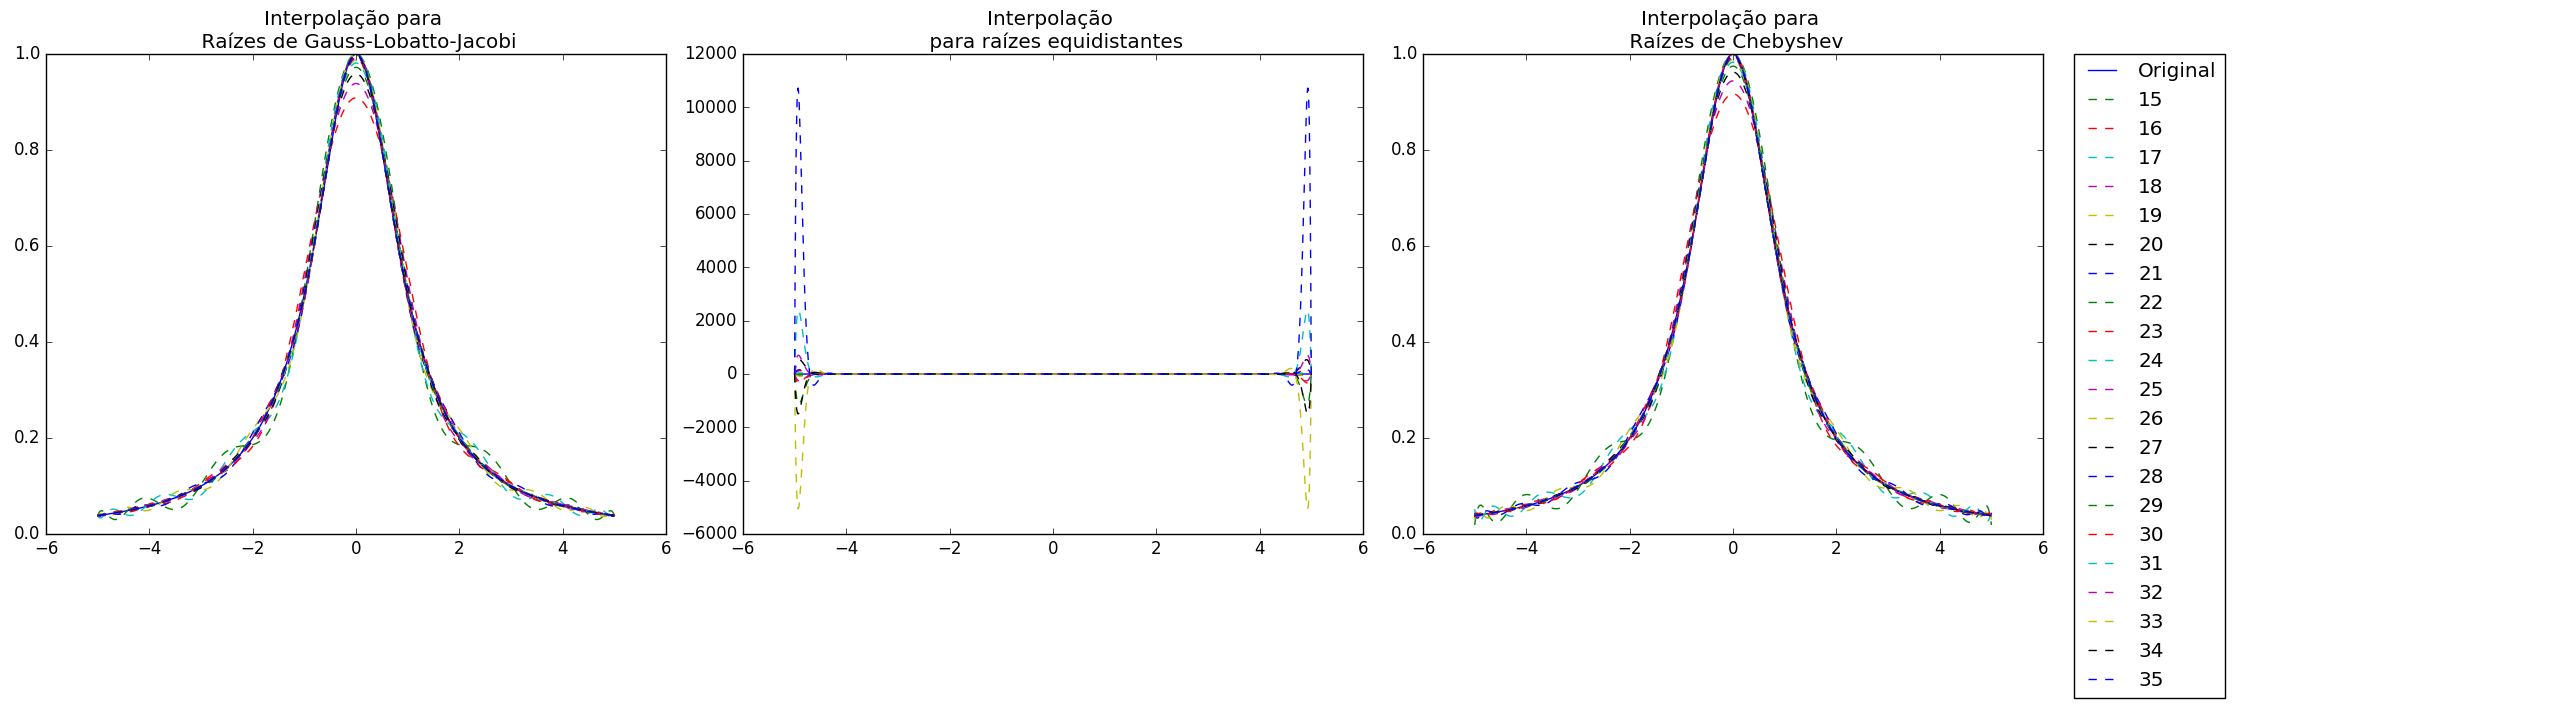
\includegraphics[width=0.8\textwidth,center]{figuras/interpolacao_todas.png}
  \caption{interpolação de polinômios de alta ordem com raízes de Gauss-Lobatto-Jacobi, igualmente espaçados, Chebyshev}
\end{figure}
Notamos novamente que para pontos igualmente espaçados a aproximação nos pontos próximos das extremidades notamos que o erro é grande, enquanto que para pontos distribuídos usando as raízes de Chebyshev e de Gauss-Lobatto-Jacobi se comportam bem nessas regiões.


\pagebreak
\begin{table}[h]
\centering
\caption{tabela de erros para os diferentes tipos de raízes}
\label{my-label}
\begin{tabular}{|l|l|l|l|}
\hline
Grau & equidist & glj       & chebyshev     \\ \hline
15   & 7.19     & 4.925e-02 & 4.660e-02 \\
16   & 2.11     & 9.128e-02 & 8.309e-02 \\
17   & 14.39    & 3.480e-02 & 3.261e-02 \\
18   & 4.22     & 6.138e-02 & 5.590e-02 \\
19   & 29.19    & 2.417e-02 & 2.249e-02 \\
20   & 8.58     & 4.126e-02 & 3.758e-02 \\
\vdots   & \vdots              & \vdots    & \vdots    \\
30   & 333.94   & 5.651e-03 & 5.154e-03 \\
31   & 2384.73  & 2.229e-03 & 2.061e-03 \\
32   & 704.08   & 3.797e-03 & 3.463e-03 \\
33   & 5058.99  & 1.510e-03 & 1.402e-03 \\
34   & 1494.38  & 2.551e-03 & 2.328e-03 \\
35   & 10719.90 & 1.025e-03 & 9.488e-04 \\ \hline
\end{tabular}
\end{table}
gráfico de erro
\begin{figure}[!ht]
  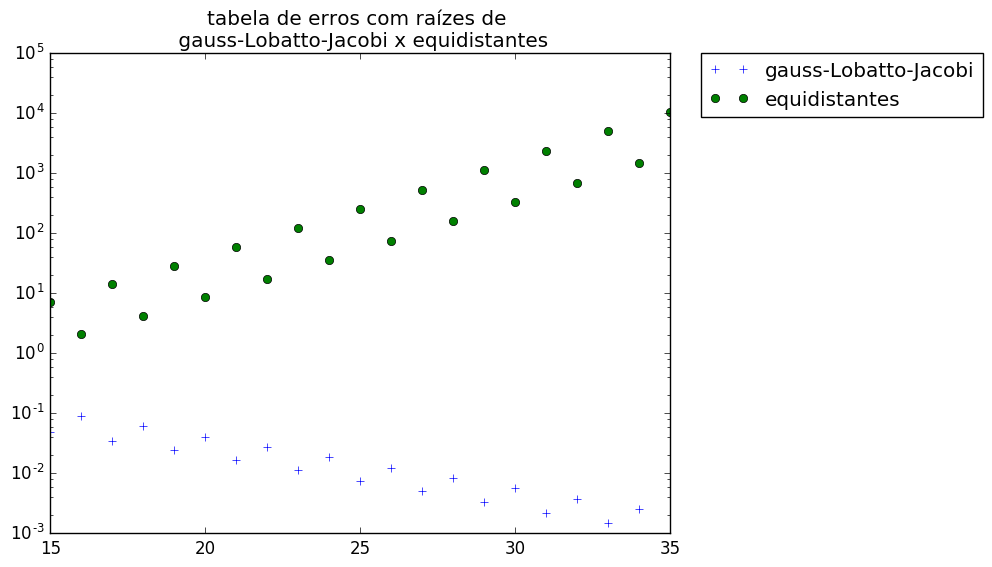
\includegraphics[width=0.5\textwidth,center]{figuras/glj_equi.png}
  \caption{comparação de erros de raízes de glj versus equidistante}
\end{figure}
\begin{figure}[!hb]
  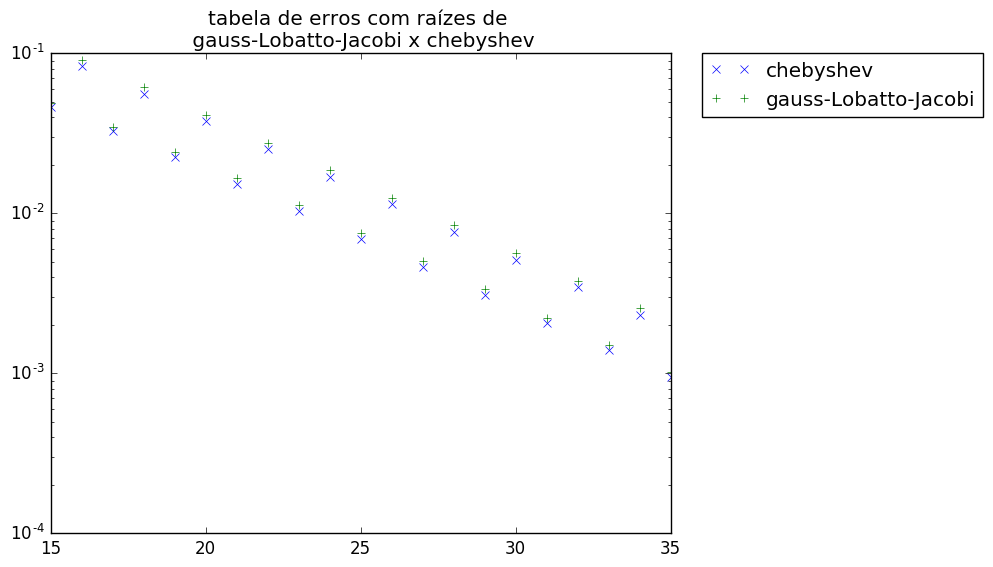
\includegraphics[width=0.5\textwidth,center]{figuras/glj_cheb.png}
  \caption{comparação de erros de raízes de glj versus equidistante}
\end{figure}

1Paragrafo paragrafo paragrafo paragrafo paragrafo paragrafo paragrafo paragrafo paragrafo paragrafo paragrafo paragrafo paragrafo paragrafo paragrafo paragrafo paragrafo paragrafo paragrafo paragrafo paragrafo paragrafo paragrafo paragrafo paragrafo paragrafo paragrafo paragrafo paragrafo paragrafo paragrafo paragrafo paragrafo paragrafo paragrafo paragrafo paragrafo paragrafo paragrafo paragrafo paragrafo
graficos de erros:


2Paragrafo paragrafo paragrafo paragrafo paragrafo paragrafo paragrafo paragrafo paragrafo paragrafo paragrafo paragrafo paragrafo paragrafo paragrafo paragrafo paragrafo paragrafo paragrafo paragrafo paragrafo paragrafo paragrafo paragrafo paragrafo paragrafo paragrafo paragrafo paragrafo paragrafo paragrafo paragrafo paragrafo paragrafo paragrafo paragrafo paragrafo paragrafo paragrafo paragrafo paragrafo


\subsection{Interpolação polinomial}

\section{Método P}

\section{Método H}


\section{Método HP}

